\chapter{Les métaux~: réactions avec les acides et corrosion}\label{ch:g9:metals-acids-corrosion}

Dans un port, la coque en acier d'un vieux bateau de pêche est striée de
\omterm{def:g9:metals-acids-corrosion:corrosion}{rouille} orange. Sur le quai, un portail recouvert de zinc est resté
trente ans sous la pluie et brille toujours d'un gris terne. Dans un
musée, une bague en or enfouie pendant trois mille ans est aussi
éclatante qu'au jour où elle a été fabriquée. Les métaux ne réagissent
pas tous de la même façon au monde qui les entoure~: certains sont
attaqués par l'eau, l'\omterm{def:g4:air-a-mixture-of-gases:air}{air} et les acides, d'autres presque pas.

\begin{recall}
Les \omterm{def:g9:ions:ion}{ions} sont des \omterm{def:g7:atoms-and-molecules:atom}{atomes} chargés~; les métaux donnent des \omterm{def:g9:ions:ion}{cations} comme
\ce{Fe^{2+}}, \ce{Zn^{2+}}, \ce{Al^{3+}}, que l'on identifie par des
tests de \omterm{def:g9:ions:precipitate}{précipitation} (\cref{ch:g9:ions}). Une \omterm{def:g9:acids-bases-ph:acidic}{solution acide} contient
beaucoup d'\omterm{def:g9:ions:ion}{ions} \ce{H+(aq)} (\cref{ch:g9:acids-bases-ph}). Le
dihydrogène \omterm{def:g4:what-a-fire-needs:burning}{brûle} avec un «~pop~» aigu à l'ouverture d'un tube à essai
(\cref{ch:g7:identifying-substances}).
\end{recall}

\begin{omfigure}
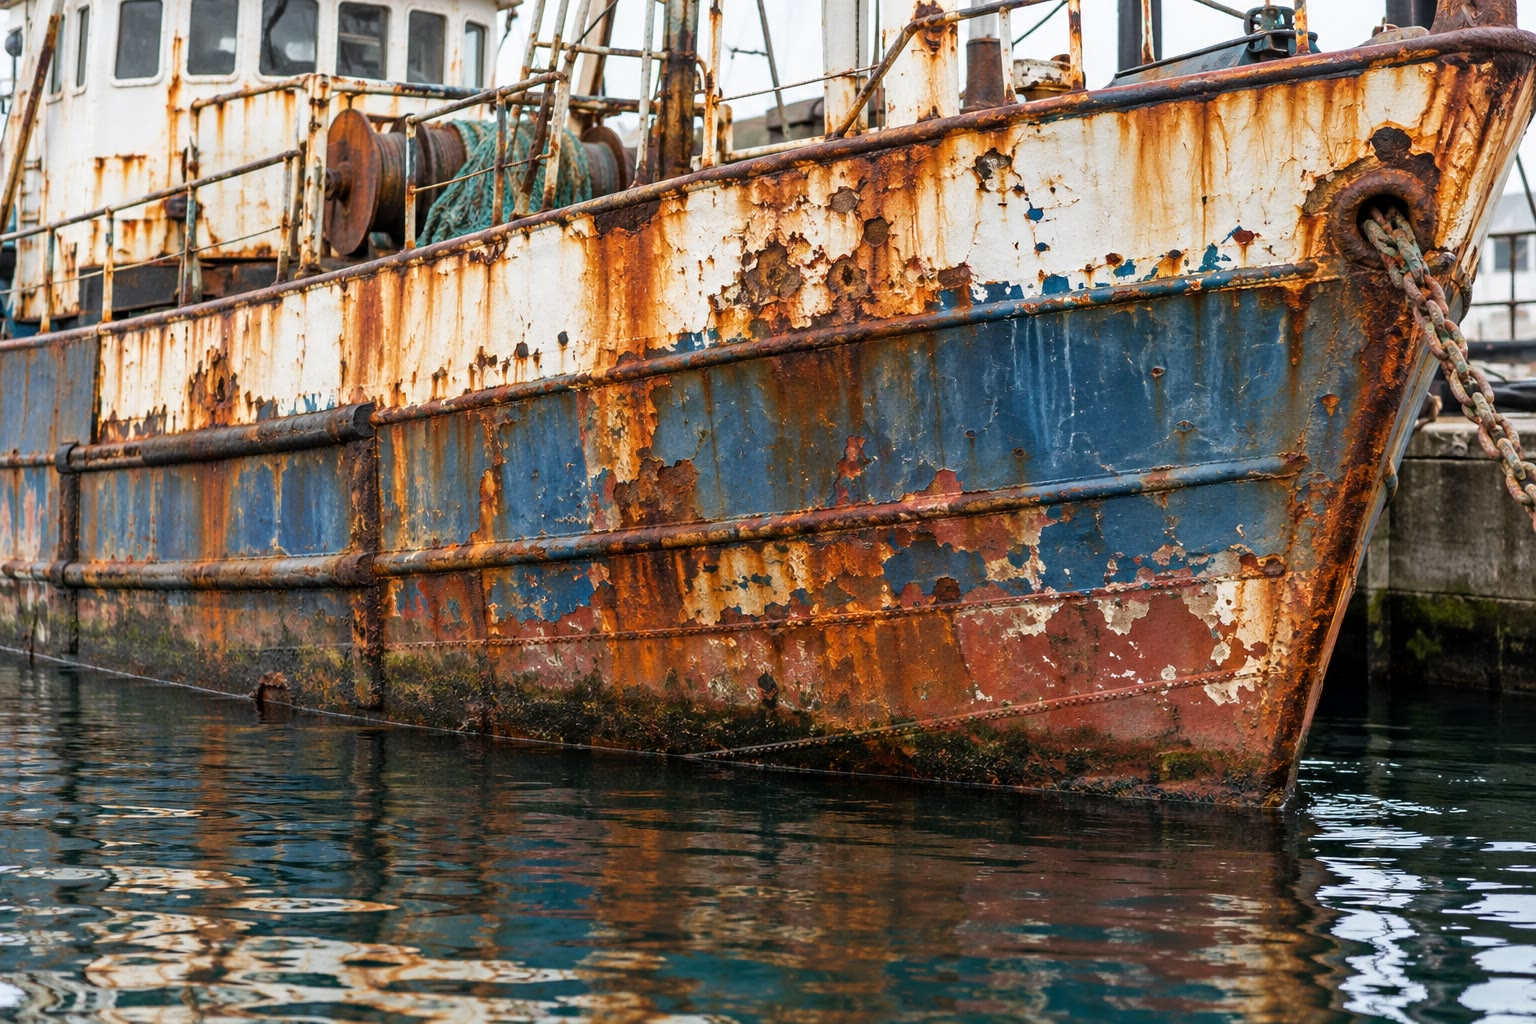
\includegraphics[width=0.55\linewidth]{images/book1/ai/g9-rusty-hull.jpg}

{\small La coque d'un vieux bateau~: l'acier \omterm{def:g9:metals-acids-corrosion:corrosion}{rouille}.}
\end{omfigure}

\section{Les métaux dans l'acide chlorhydrique}

\begin{inthelab}[Trois métaux dans l'acide]
L'enseignant met un petit morceau de fer, de zinc et de cuivre dans
trois tubes à essai d'acide chlorhydrique dilué. Des bulles montent du
fer et du zinc, lentement pour le fer, vivement pour le zinc, et les
métaux disparaissent peu à peu~; rien ne se passe avec le cuivre. Le
gaz, recueilli dans un petit tube, produit un «~pop~» aigu~: c'est du
dihydrogène. Avec l'hydroxyde de sodium, le liquide du premier tube
donne un \omterm{def:g9:ions:precipitate}{précipité} vert (\omterm{def:g9:ions:ion}{ions} \ce{Fe^{2+}}), celui du deuxième un
\omterm{def:g9:ions:precipitate}{précipité} blanc (\omterm{def:g9:ions:ion}{ions} \ce{Zn^{2+}}).
\end{inthelab}

\begin{omfigure}
\begin{tikzpicture}[font=\small, scale=1.2]
  \foreach \k/\m/\c/\bub in {0/fer/black!45/4, 1/zinc/black!25/9, 2/cuivre/orange!60!brown/0} {
    \pic[transform shape] at (\k*2.4,0) {testtube={0.55}{omWater!70}};
    \fill[\c] (\k*2.4-0.13,0.08) rectangle (\k*2.4+0.13,0.35);
    \ifnum\bub>0
      \foreach \j in {1,...,\bub} {
        \pgfmathsetmacro\yy{0.45+0.12*\j}
        \pgfmathsetmacro\xx{\k*2.4+0.1*sin(97*\j)}
        \draw[black!55] (\xx,\yy) circle (0.035);
      }
    \fi
    \node[anchor=north, align=center] at (\k*2.4,-0.15) {\m};
  }
  \node[anchor=north, align=center, font=\footnotesize] at (0,-0.6) {bulles,\\ lentement};
  \node[anchor=north, align=center, font=\footnotesize] at (2.4,-0.6) {bulles,\\ vivement};
  \node[anchor=north, align=center, font=\footnotesize] at (4.8,-0.6) {pas de\\ réaction};
\end{tikzpicture}

{\small Le fer, le zinc et le cuivre dans l'acide chlorhydrique dilué~:
le fer et le zinc dégagent du dihydrogène~; le cuivre ne réagit pas.}
\end{omfigure}

\begin{proposition}[Métal et acide]\label{prop:g9:metals-acids-corrosion:acid}
Beaucoup de métaux --- le fer, le zinc, l'aluminium, le magnésium ---
réagissent avec les \omterm{def:g9:ions:ion}{ions} \ce{H+} d'un acide~: le métal disparaît sous
forme d'\omterm{def:g9:ions:ion}{ions} métalliques, qui restent dissous, et du dihydrogène gazeux
se dégage. Le cuivre, l'argent et l'or ne réagissent pas avec l'acide
chlorhydrique.
\end{proposition}

\section{Écrire l'équation avec les ions}

\begin{definition}[Ion spectateur]\label{def:g9:metals-acids-corrosion:spectator}
Un \omterm{def:g9:ions:ion}{ion} présent dans une solution pendant une réaction, mais qui n'y
participe pas et se retrouve inchangé à la fin, est un \emph{ion
spectateur}\index{ion spectateur}. On ne l'écrit pas dans l'équation.
\end{definition}

\begin{example}[Le fer et le zinc dans l'acide chlorhydrique]\label{ex:g9:metals-acids-corrosion:iron}
L'acide chlorhydrique contient des \omterm{def:g9:ions:ion}{ions} \ce{H+(aq)} et \ce{Cl-(aq)}. Les
\omterm{def:g9:ions:ion}{ions} chlorure se retrouvent inchangés à la fin~: ce sont des
spectateurs. Les équations sont
\[
  \ce{Fe(s) + 2H+(aq) -> Fe^{2+}(aq) + H2(g)}, \qquad
  \ce{Zn(s) + 2H+(aq) -> Zn^{2+}(aq) + H2(g)}.
\]
Elles sont ajustées à la fois pour les \omterm{def:g7:atoms-and-molecules:atom}{atomes} et pour les charges~:
$+2$ de chaque côté.
\end{example}

\begin{method}[Écrire l'équation de la réaction d'un métal avec un acide]\label{met:g9:metals-acids-corrosion:write}
\begin{enumerate}
  \item \omterm{def:g7:chemical-reactions:reactant}{Réactifs}~: le métal (s) et les \omterm{def:g9:ions:ion}{ions} \ce{H+(aq)}.
  \item Produits~: l'\omterm{def:g9:ions:ion}{ion} métallique (aq), avec sa charge habituelle, et
        le dihydrogène \ce{H2(g)}.
  \item Ajuster les \omterm{def:g7:atoms-and-molecules:atom}{atomes}, puis vérifier que la charge totale est la
        même des deux côtés.
\end{enumerate}
Pour l'aluminium~: \ce{2Al(s) + 6H+(aq) -> 2Al^{3+}(aq) + 3H2(g)}~;
charge $+6$ de chaque côté.
\end{method}

\begin{safety}{\ghs[0.8cm]{GHS02}\ghs[0.8cm]{GHS04}}
% ledger: ghs:H2
Le dihydrogène dégagé est extrêmement inflammable. La réaction est
réalisée dans de petits tubes à essai, par l'enseignant, loin de toute
flamme autre que celle du test du «~pop~».
\end{safety}

\section{La corrosion}

\begin{definition}[Corrosion et rouille]\label{def:g9:metals-acids-corrosion:corrosion}
La \emph{corrosion}\index{corrosion} est l'attaque lente d'un métal par
les substances qui l'entourent --- dioxygène, eau, acides, sels --- qui
transforme le métal en \omterm{def:g9:ions:ion}{ions} ou en composés comme des oxydes. La corrosion
du fer et de l'acier produit la \emph{rouille}\index{rouille}, un oxyde
de fer hydraté, brun et friable, qui s'écaille et laisse l'attaque se
poursuivre en profondeur.
\end{definition}

\begin{proposition}[Ce dont le fer a besoin pour rouiller]\label{prop:g9:metals-acids-corrosion:needs}
Le fer ne \omterm{def:g9:metals-acids-corrosion:corrosion}{rouille} que lorsque le dioxygène et l'eau l'atteignent tous
les deux. Du sel dissous dans l'eau, comme sur les routes salées en
hiver ou au bord de la mer, accélère la \omterm{def:g9:metals-acids-corrosion:corrosion}{rouille}.
\end{proposition}

\begin{inthelab}[Trois clous, une semaine]
On place trois clous en fer propres dans trois tubes à essai~: le
premier dans de l'\omterm{def:g4:air-a-mixture-of-gases:air}{air} sec avec un desséchant qui retire la vapeur
d'eau~; le deuxième dans de l'eau bouillie pour en chasser l'\omterm{def:g4:air-a-mixture-of-gases:air}{air}
dissous, recouverte d'une couche d'huile~; le troisième à moitié dans
l'eau du robinet, à moitié dans l'\omterm{def:g4:air-a-mixture-of-gases:air}{air}. Au bout d'une semaine, seul le
troisième clou est rouillé.
\end{inthelab}

\begin{omfigure}
\begin{tikzpicture}[font=\small, scale=1.2]
  % tube 1: dry air, drying agent
  \pic[transform shape] at (0,0) {testtube={0.18}{white!80!black}};
  \foreach \x/\y in {-0.12/0.15,0.08/0.12,-0.02/0.3,0.12/0.32,-0.14/0.42,0.03/0.48}
    \fill[black!35] (\x,\y) circle (0.05);
  \fill[black!45] (-0.03,1.0) rectangle (0.03,2.4);
  \fill[black!45] (-0.09,2.4) rectangle (0.09,2.48);
  \fill[black!60] (-0.3,2.8) rectangle (0.3,3.1);
  \node[anchor=north, align=center] at (0,-0.15) {air sec~:\\ pas de rouille};
  % tube 2: boiled water under oil
  \pic[transform shape] at (2.6,0) {testtube={0.7}{omWater!80}};
  \fill[yellow!55!orange!60] (2.36,1.85) rectangle (2.84,2.1);
  \fill[black!45] (2.57,0.3) rectangle (2.63,1.7);
  \fill[black!45] (2.51,1.7) rectangle (2.69,1.78);
  \fill[black!60] (2.3,2.8) rectangle (2.9,3.1);
  \node[anchor=north, align=center] at (2.6,-0.15) {eau sans air~:\\ pas de rouille};
  % tube 3: water and air
  \pic[transform shape] at (5.2,0) {testtube={0.4}{omWater!80}};
  \fill[black!45] (5.17,0.3) rectangle (5.23,2.2);
  \fill[black!45] (5.11,2.2) rectangle (5.29,2.28);
  \fill[orange!60!brown] (5.15,0.9) rectangle (5.25,1.5);
  \node[anchor=north, align=center] at (5.2,-0.15) {eau et air~:\\ rouille};
  \draw[<-, omProp, thick] (-0.15,0.3) -- (-0.9,0.7) node[left, text=black, font=\footnotesize] {desséchant};
  \draw[<-, omProp, thick] (2.85,1.98) -- (3.6,2.4) node[right, text=black, font=\footnotesize] {huile};
\end{tikzpicture}

{\small L'expérience des trois clous~: le fer ne \omterm{def:g9:metals-acids-corrosion:corrosion}{rouille} que là où l'eau
et le dioxygène l'atteignent ensemble, ici à la surface de l'eau.}
\end{omfigure}

\begin{example}[L'aluminium et le cuivre se protègent eux-mêmes]\label{ex:g9:metals-acids-corrosion:protect}
L'aluminium est attaqué aussitôt par le dioxygène de l'\omterm{def:g4:air-a-mixture-of-gases:air}{air}, mais la fine
couche d'oxyde formée adhère au métal et l'isole de l'\omterm{def:g4:air-a-mixture-of-gases:air}{air}~: les cadres
de fenêtre en aluminium durent des dizaines d'années. Le cuivre,
lentement attaqué par l'\omterm{def:g4:air-a-mixture-of-gases:air}{air}, l'eau et le dioxyde de carbone, se couvre
d'une croûte verte, la patine, qui adhère elle aussi et protège le métal
au-dessous. La \omterm{def:g9:metals-acids-corrosion:corrosion}{rouille}, au contraire, s'écaille.
\end{example}

\begin{omfigure}
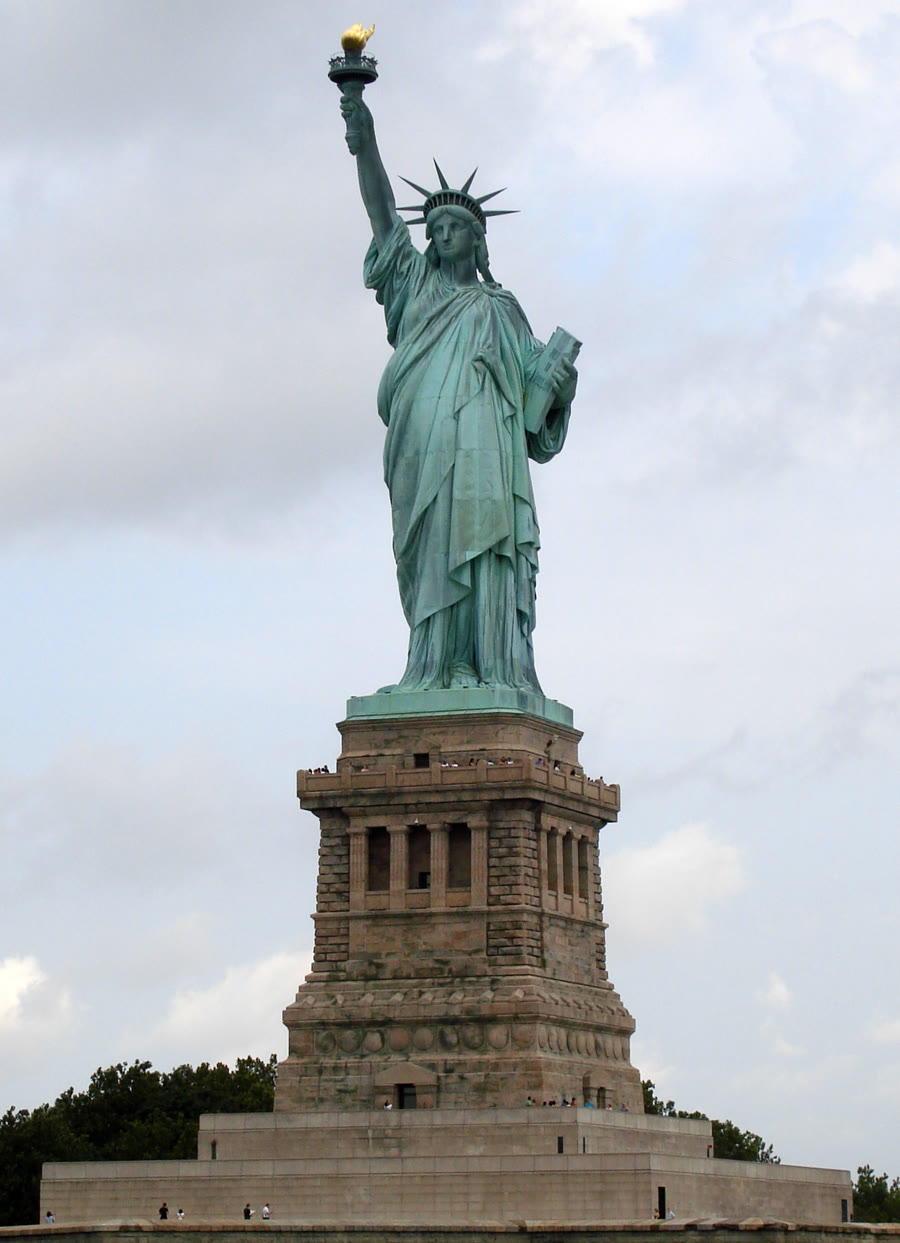
\includegraphics[height=6cm]{images/book1/statue-patina.jpg}

{\small La statue de la Liberté~: sa peau de cuivre est couverte d'une
patine verte. Photo~: Elcobbola, domaine public.}
\end{omfigure}

\section{Protéger les métaux}

\begin{definition}[Galvanisation]\label{def:g9:metals-acids-corrosion:galvanising}
La \emph{galvanisation}\index{galvanisation} consiste à recouvrir l'acier
d'une couche de zinc, en le plongeant dans du zinc fondu. Le zinc est
attaqué par l'\omterm{def:g4:air-a-mixture-of-gases:air}{air} et l'eau à la place de l'acier qu'il recouvre~: même là
où le revêtement est rayé, le zinc voisin est corrodé en premier et
l'acier est épargné.
\end{definition}

\begin{proposition}[Les moyens de protéger le fer et l'acier]\label{prop:g9:metals-acids-corrosion:ways}
\begin{itemize}
  \item tenir l'eau et l'\omterm{def:g4:air-a-mixture-of-gases:air}{air} à distance~: peinture, huile, graisse,
        revêtement plastique~;
  \item galvaniser~: une couche de zinc qui se corrode à la place de
        l'acier~;
  \item utiliser de l'acier inoxydable, un alliage de fer et de chrome,
        qui se protège lui-même par une fine couche d'oxyde étanche~;
  \item fixer des blocs de zinc sur les coques des navires~: le zinc est
        lentement rongé à la place de l'acier, et on le remplace de temps
        en temps (le fonctionnement de ce procédé est expliqué dans un
        volume universitaire).
\end{itemize}
\end{proposition}

\begin{omfigure}
\begin{minipage}[b]{0.52\linewidth}\centering
\begin{tikzpicture}[font=\small]
  \fill[black!35] (0,0) rectangle (5,0.8);
  \fill[black!15] (0,0.8) rectangle (2.2,1.1);
  \fill[black!15] (2.8,0.8) rectangle (5,1.1);
  \fill[omWater!80] (1.6,1.1) rectangle (3.4,1.35);
  \fill[omWater!80] (2.2,0.8) rectangle (2.8,1.1);
  \draw[black!60] (0,0) rectangle (5,0.8);
  \foreach \x in {1.95,2.1} \draw[->, omProp, thick] (\x,1.25) -- (\x+0.05,1.7);
  \node[anchor=west, font=\footnotesize] at (5.1,0.4) {acier};
  \node[anchor=west, font=\footnotesize] at (5.1,0.95) {couche de zinc};
  \node[anchor=south, font=\footnotesize, align=center] at (2.0,1.75) {des ions zinc\\ passent dans l'eau};
  \node[anchor=north, font=\footnotesize, align=center] at (2.5,-0.05) {une rayure~: l'acier\\ est mis à nu, mais le zinc\\ autour se corrode d'abord};
\end{tikzpicture}

{\small Une tôle galvanisée rayée.}
\end{minipage}\hfill
\begin{minipage}[b]{0.44\linewidth}\centering
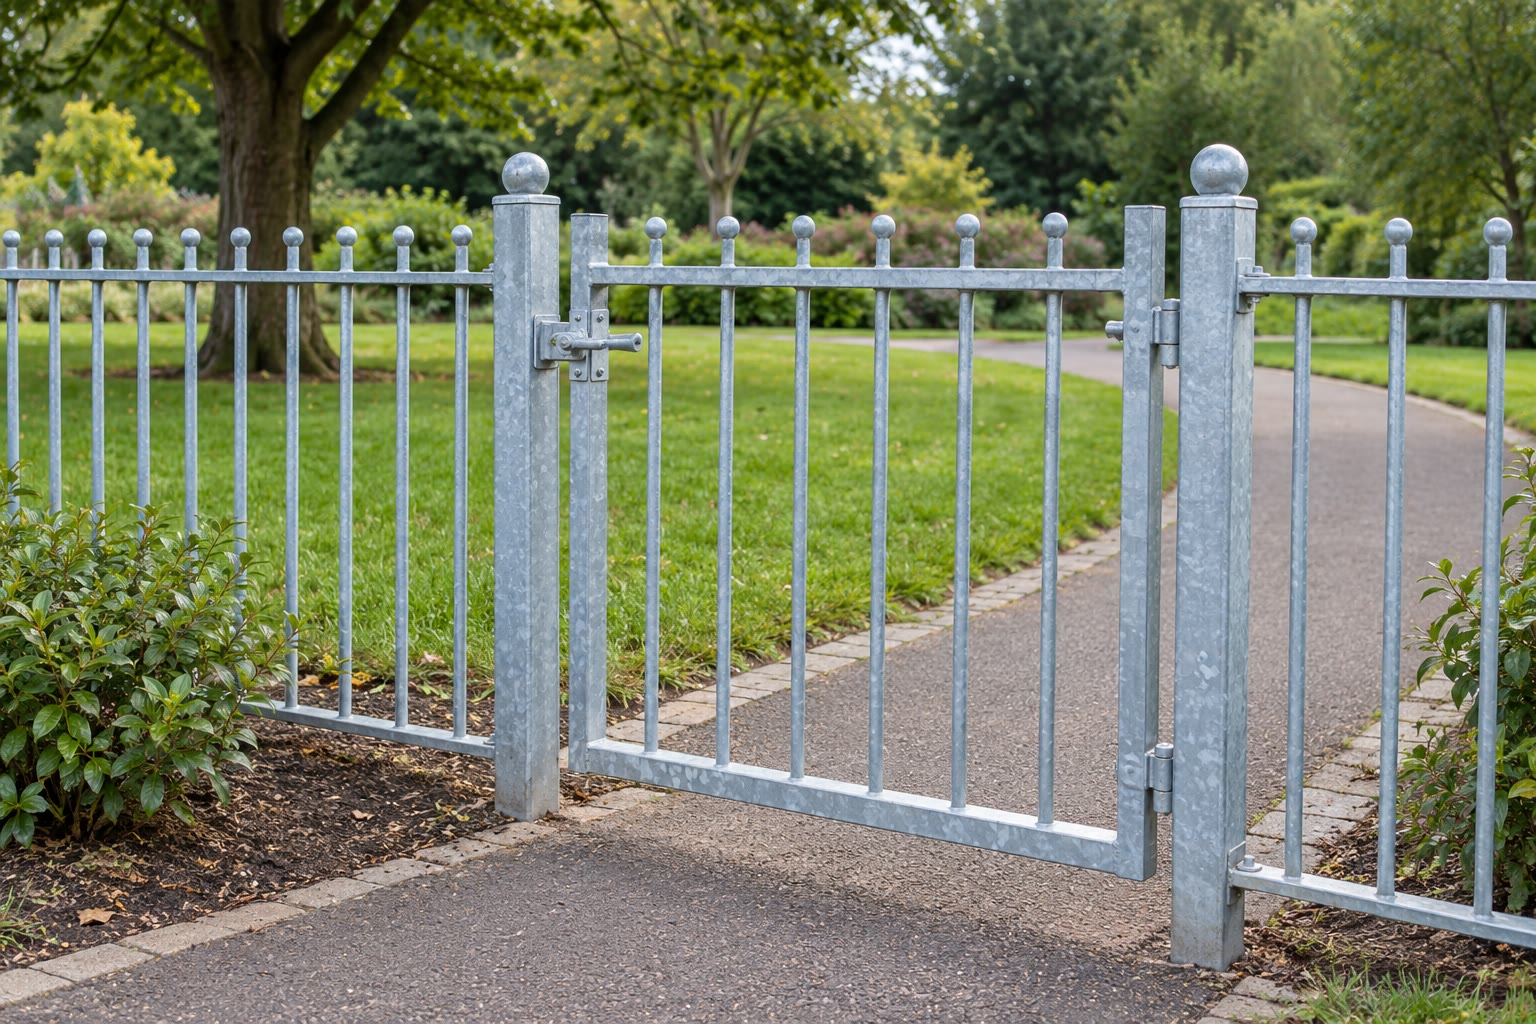
\includegraphics[width=\linewidth,height=4.4cm,keepaspectratio]{images/book1/ai/g9-galvanised-railings.jpg}

{\small Une rambarde en acier galvanisé.}
\end{minipage}
\end{omfigure}

\section{Exercices}

\begin{exercise}[$\star$]\label{exo:g9:metals-acids-corrosion:1}
Quel gaz se dégage quand le zinc réagit avec l'acide chlorhydrique~?
Comment l'identifie-t-on~?
\end{exercise}

\begin{exercise}[$\star$]\label{exo:g9:metals-acids-corrosion:2}
Lesquels de ces métaux réagissent avec l'acide chlorhydrique dilué~: le
fer, le cuivre, le zinc, l'or, l'aluminium~?
\end{exercise}

\begin{exercise}[$\star$]\label{exo:g9:metals-acids-corrosion:3}
De quoi le fer a-t-il besoin pour rouiller~?
\end{exercise}

\begin{exercise}[$\star$]\label{exo:g9:metals-acids-corrosion:4}
Qu'est-ce qu'un \omterm{def:g9:metals-acids-corrosion:spectator}{ion spectateur}~? Nomme l'\omterm{def:g9:metals-acids-corrosion:spectator}{ion spectateur} quand le fer
réagit avec l'acide chlorhydrique.
\end{exercise}

\begin{exercise}[$\star\star$]\label{exo:g9:metals-acids-corrosion:5}
Écris l'équation de la réaction du magnésium avec les \omterm{def:g9:ions:ion}{ions} \ce{H+} d'un
acide (l'\omterm{def:g9:ions:ion}{ion} magnésium est \ce{Mg^{2+}}). Vérifie les charges.
\end{exercise}

\begin{exercise}[$\star\star$]\label{exo:g9:metals-acids-corrosion:6}
Après la réaction du fer avec l'acide chlorhydrique, comment peux-tu
montrer que la solution contient des \omterm{def:g9:ions:ion}{ions} fer(II)~?
\end{exercise}

\begin{exercise}[$\star\star$]\label{exo:g9:metals-acids-corrosion:7}
Regarde la figure des trois clous. Pourquoi l'eau du deuxième tube
est-elle bouillie et recouverte d'huile~?
\end{exercise}

\begin{exercise}[$\star\star$]\label{exo:g9:metals-acids-corrosion:8}
Pourquoi une voiture rouille-t-elle plus vite dans une ville où l'on
sale les routes en hiver~?
\end{exercise}

\begin{exercise}[$\star\star$]\label{exo:g9:metals-acids-corrosion:9}
Pourquoi les cadres de fenêtre en aluminium ne disparaissent-ils pas
par \omterm{def:g9:metals-acids-corrosion:corrosion}{corrosion}, alors que l'aluminium réagit avec le dioxygène de
l'\omterm{def:g4:air-a-mixture-of-gases:air}{air}~?
\end{exercise}

\begin{exercise}[$\star\star$]\label{exo:g9:metals-acids-corrosion:10}
Donne trois moyens de protéger un cadre de vélo en acier contre la
\omterm{def:g9:metals-acids-corrosion:corrosion}{rouille}.
\end{exercise}

\begin{exercise}[$\star\star\star$]\label{exo:g9:metals-acids-corrosion:11}
Écris et vérifie l'équation de la réaction de l'aluminium avec les \omterm{def:g9:ions:ion}{ions}
\ce{H+} d'un acide. Combien de \omterm{def:g7:atoms-and-molecules:molecule}{molécules} de dihydrogène se forment pour
200 \omterm{def:g7:atoms-and-molecules:atom}{atomes} d'aluminium~?
\end{exercise}

\begin{exercise}[$\star\star\star$]\label{exo:g9:metals-acids-corrosion:12}
Un seau en acier galvanisé est rayé jusqu'à l'acier. Explique pourquoi
l'acier au fond de la rayure ne \omterm{def:g9:metals-acids-corrosion:corrosion}{rouille} pas avant longtemps.
\end{exercise}

\section{Problème~: quelle épaisseur de zinc~?}

\begin{problem}[{Problème du week-end --- dissoudre le revêtement de zinc
d'une plaque galvanisée pour connaître son épaisseur}]
\label{pb:g9:metals-acids-corrosion:1}
% ledger: rho:Zn
Une plaque d'acier galvanisé, un carré de \qty{10.0}{cm} de côté, est
recouverte de zinc sur ses deux faces (on néglige les tranches). Au
laboratoire, l'enseignant la pèse, \qty{125.6}{g}, puis la plonge dans
de l'acide chlorhydrique contenant un additif qui empêche l'acide
d'attaquer l'acier. Quand l'effervescence s'arrête, la plaque est
rincée, séchée et pesée de nouveau~: \qty{113.5}{g}. La masse de
\qty{1}{cm^3} de zinc est \qty{7.13}{g}.

\medskip
\noindent\textbf{Partie I --- La réaction.}
\begin{enumerate}
  \item Écris l'équation de la réaction du zinc avec les \omterm{def:g9:ions:ion}{ions} \ce{H+} de
        l'acide.
  \item Quel gaz provoque l'effervescence~? Décris son test.
  \item Quel test montrerait ensuite les \omterm{def:g9:ions:ion}{ions} zinc dans la solution~?
  \item Nomme les \omterm{def:g9:metals-acids-corrosion:spectator}{ions spectateurs}.
\end{enumerate}

\medskip
\noindent\textbf{Partie II --- Le zinc.}
\begin{enumerate}[resume]
  \item Quelle masse de zinc s'est dissoute~?
  \item Pourquoi l'effervescence est-elle le signe que tout le zinc n'est
        pas encore dissous~?
  \item Que deviendrait l'acier si l'acide ne contenait pas l'additif~?
        Quel test le montrerait alors~?
  \item Pourquoi le zinc protège-t-il l'acier de la plaque tant qu'il est
        présent~?
\end{enumerate}

\medskip
\noindent\textbf{Partie III --- L'épaisseur.}
\begin{enumerate}[resume]
  \item Quelle est l'aire totale recouverte de la plaque, en
        \unit{cm^2}~?
  \item Quel volume le zinc occupait-il~?
  \item Déduis-en l'épaisseur de la couche de zinc, en centimètres.
  \item Exprime cette épaisseur en micromètres
        (\qty{1}{cm} $= \qty{10000}{\micro m}$).
\end{enumerate}
\end{problem}
